\documentclass[a4paper]{llncs}

\usepackage[utf8]{inputenc}
\usepackage[colorinlistoftodos, textwidth=35mm, textsize=footnotesize]{todonotes}
\usepackage[pdftex,breaklinks,bookmarks,bookmarksnumbered,plainpages=false,pdfpagelabels,hyperindex]{hyperref}
\usepackage{url}
\usepackage[space]{cite}
\usepackage{footnote}
\usepackage{amsmath}

\newcommand{\squishlist}{ 
   \begin{list}{$\bullet$}
    { \setlength{\itemsep}{0pt}      \setlength{\parsep}{3pt} 
      \setlength{\topsep}{3pt}       \setlength{\partopsep}{0pt}
      \setlength{\leftmargin}{1.5em} \setlength{\labelwidth}{1em}
      \setlength{\labelsep}{0.5em} } }

\newcommand{\squishend}{
  \end{list}  }

\newcommand{\simos}[1]{\todo[color=green!30,caption={}]{\textbf{Simos} #1}}
\newcommand{\usman}[1]{\todo[color=orange!70,caption={}]{\textbf{Usman} #1}}

\newcommand{\comment}[1]{\todo[inline,color=red!30,caption={}]{#1}}
\newcommand{\commentBox}[1]{\todo[noinline,color=red!30,caption={}]{#1}}
\newcommand{\textBlue}[1]{\textcolor{blue}{#1}}

\newcommand{\approach}{ENTRUST}

\begin{document}
\title{\approach: Engineering Trustworthy Self-Managing Systems -- Technical Report}
\author{}
\institute{}
\maketitle

%\begin{Abstract}
%\end{Abstract}

%%%%%%%%%%%%%%%%%%%%%%%%%%%%%%%%%%
%\vspace*{-5mm}
\section{INTRODUCTION} \label{sec:introduction}
%!TEX root = ../ENTRUST_TR.tex

%This section will explain what are we going to do, which is combining two technologies ActivFORMS + Prism.
%\simos{References needed}
The increasing complexity of software systems combined with the need to develop more versatile, resilient, and reliable systems instigated the vision of self-managing systems, also known as autonomous computing\cite{Kephart2003:Comp, Ganek2003:IBM}. In this regard, self-managing systems are expected not only to operate with minimal administrator intervention throughout their lifetime, but also to adapt while providing service in response to environment changes, evolving requirements and unexpected failures. As a result, the software engineering research community devoted much effort in developing frameworks, methodologies and architectures that support the engineering of systems enhanced with self-* capabilities (e.g., self-adaptive, self-managing, self-healing, self-optimising);~see \cite{Salehie2009:TAAS, Huebscher2008:ACM} for more information. 

Despite the research progress achieved since the advent of autonomous computing, the engineering of trustworthy self-managing systems remains a major research challenge. This barrier constrains the applicability of self-managing systems in safety-critical and business-critical applications, as for example, in healthcare, e-commerce, defence and finance. Systems deployed in these application areas should work dependably and must be characterised by high-integrity runtime operation, as defined by NIST~\cite{NIST}: ``High integrity software is software that must be trusted to work dependably in some critical function, and whose failure to do so may have catastrophic results, such as serious injury, loss of life or property, business failure or breach of security."

The software engineering community classified the provision of evidence, i.e., assurances, that a system operates dependably throughout its lifetime among the most important research objectives for self-managing systems~\cite{Cheng2009:Dagstuhl}. In fact, assurances was amid the research threads highlighted in the most recent roadmaps for self-adaptive systems~\cite{Lemos2013:Dagstuhl, Lemos2014:Dagstuhl}. We define assurances as \textit{``the provision of evidence that the system satisfies its stated functional and non-functional requirements during its operation in the presence of self- adaptation"}~\cite{Lemos2014:Dagstuhl}.

In this work, we extend the current practices on the provision of assurances for self-managing systems. To this end, we introduce the first tool-supported methodology for assuring the safety of the closed control loops of self-managing systems using established industry practices. Our framework for the ENgineering of TRUstworthy Self-managing sysTems (\approach) integrates:
\squishlist
	\item an extended version of our approach to developing formally verified monitor-analysis-planning-execution (MAPE) autonomic control loops~\cite{Iftikhar2014:SEAMS};
	\item our runtime quantitative verification technique for the analysis stage of these loops~\cite{Calinescu2012:CACM};
	\item an industry-adopted approach to arguing security~\cite{Weinstock2007} based on the widely used Goal Structuring Notation (GSN) for safety arguments~\cite{Kelly2004:DSN}.
\squishend

The report is organised as follows.  Section~\ref{sec:example} describes the self-adaptive unmanned marine vehicle embedded system used for illustrating and evaluating \approach. Sections~\ref{sec:activForms} and~\ref{sec:rqv} introduces the approaches underpinning \approach, while Section~\ref{sec:implementation} presents the realisation of \approach\ for the implementation of the embedded system described in Section~\ref{sec:example}..

%The theoretical background underpinning \approach\ is introduced in Section~\ref{sec:preliminaries}, while Section~\ref{sec:entrust} describes the \approach\ methodology, and 


%%%%%%%%%%%%%%%%%%%%%%%%%%%%%%%%%%
%\vspace*{-15mm}
\section{Running Example}\label{sec:example}
%!TEX root = ../ENTRUST_TR.tex

We will demonstrate the application of \approach\ using a self-adaptive UUV embedded system, adapted from~\cite{Gerasimou2014:SEAMS}. UUVs are increasingly used in a wide range of oceanographic and military tasks, including oceanic surveillance (e.g., to monitor pollution levels and ecosystems), undersea mapping, and mine detection. Limitations intrinsic to the environment in which these vehicles operate (e.g., impossibility  to maintain UUV-operator communication during missions and high frequency of unexpected changes) require that UUV systems are self-adaptive. These systems are also safety critical (e.g., when used for mine detection and surveillance of ecosystems that should not be impacted) and/or business critical, since UUVs are often expensive equipment that should not be lost during missions.

The self-adaptive system in our study consists of a UUV deployed to carry out a data gathering mission. The UUV is equipped with $n \geq 1$ on-board sensors that can measure the same characteristic of the ocean environment (e.g., water current, salinity or temperature). When used, the sensors take measurements with different, variable rates $r_1$, $r_2$, \ldots, $r_n$. The probability that each sensor produces measurements that are sufficiently accurate for the purpose of the mission depends on the UUV speed $sp$, given by  $p_1$, $p_2$, \ldots, $p_n$\footnote{This information can be extracted from the technical specification of sensors; for example, see \url{http://www.ashtead-technology.com/rental-equipment/teledyne-rdi-600khz-navigator/}}. For each measurement taken, different amount of energy is consumed, given by $e_1$, $e_2$, \ldots, $e_n$. % These measurements have an accuracy that depends on the UUV speed $sp$, and the (speed-dependent) probabilities $p_1$, $p_2$, \ldots, $p_n$ that the sensors produce measurements that are sufficiently accurate for the purpose of mission can be calculated from the technical specifications of the sensors. 
Finally, the $n$ sensors can be switched on and off individually (e.g., to save battery power when not required), but these operations consume an amount of energy given by $e^\mathrm{on}_1$, $e^\mathrm{on}_2$, \ldots, $e^\mathrm{on}_n$ and $e^\mathrm{off}_1$, $e^\mathrm{off}_2$, \ldots, $e^\mathrm{off}_n$, respectively.

The UUV is required to self-adapt to changes in the observed sensor measurement rates $r_i$, $1\leq i\leq n$, and to sensor failures by dynamically adjusting:
\squishlist
\item[(a)] the UUV speed $sp$
\item[(b)] the sensor configuration $x_1$, $x_2$, \ldots, $x_n$ (where $x_i=1$ if the $i$-th sensor is on and $x_i=0$ otherwise)
\squishend
so that the UUV complies with the following requirements at all times:
\squishlist
	\item[\textbf{R1}:] The UUV should take at least 20 measurements of sufficient accuracy for every 10~metres of mission distance.
	\item[\textbf{R2}:] The energy consumption of the sensors should not exceed 120 Joules per 10 surveyed metres.
	\item[\textbf{R3}:] If requirements R1 and R2 are satisfied by multiple configurations, the UUV should use one of these configurations that minimises the cost function
\begin{equation}
\label{eq:cost}
cost = w_1 E + w_2 s^{-1},
\end{equation}
where $E$ represents the energy consumed by the sensors to survey a 10m mission distance, and $w_1, w_2 >0$ represent weights that reflect the relative importance of carrying out the mission with reduced battery usage and completing the mission faster.
\squishend

%%%%%%%%%%%%%%%%%%%%%%%%%%%%%%%%%%
\section{ActivFORMS}\label{sec:activForms}
%!TEX root = ../ENTRUST_TR.tex
ActivFORMS is a formal approach for self-adaptation that uses an integrated formal model of the adaptive components and knowledge models. The formal model is executed directly by a virtual machine to realize adaptation, hence called active model. ActivFORMS approach distinguishes itself from existing approaches in two ways. First, the formally verified model of the complete feedback loop is directly executed by the virtual machine, which guarantees the verified adaptation goals at runtime. As the active model is directly executed by ActivFORMS, the approach does not require coding. Second, ActivFORMS supports dynamic change of the active model. A new feedback loop model can be deployed at runtime to meet new or changing goals. 

\begin{figure}[b!]
	\centering
	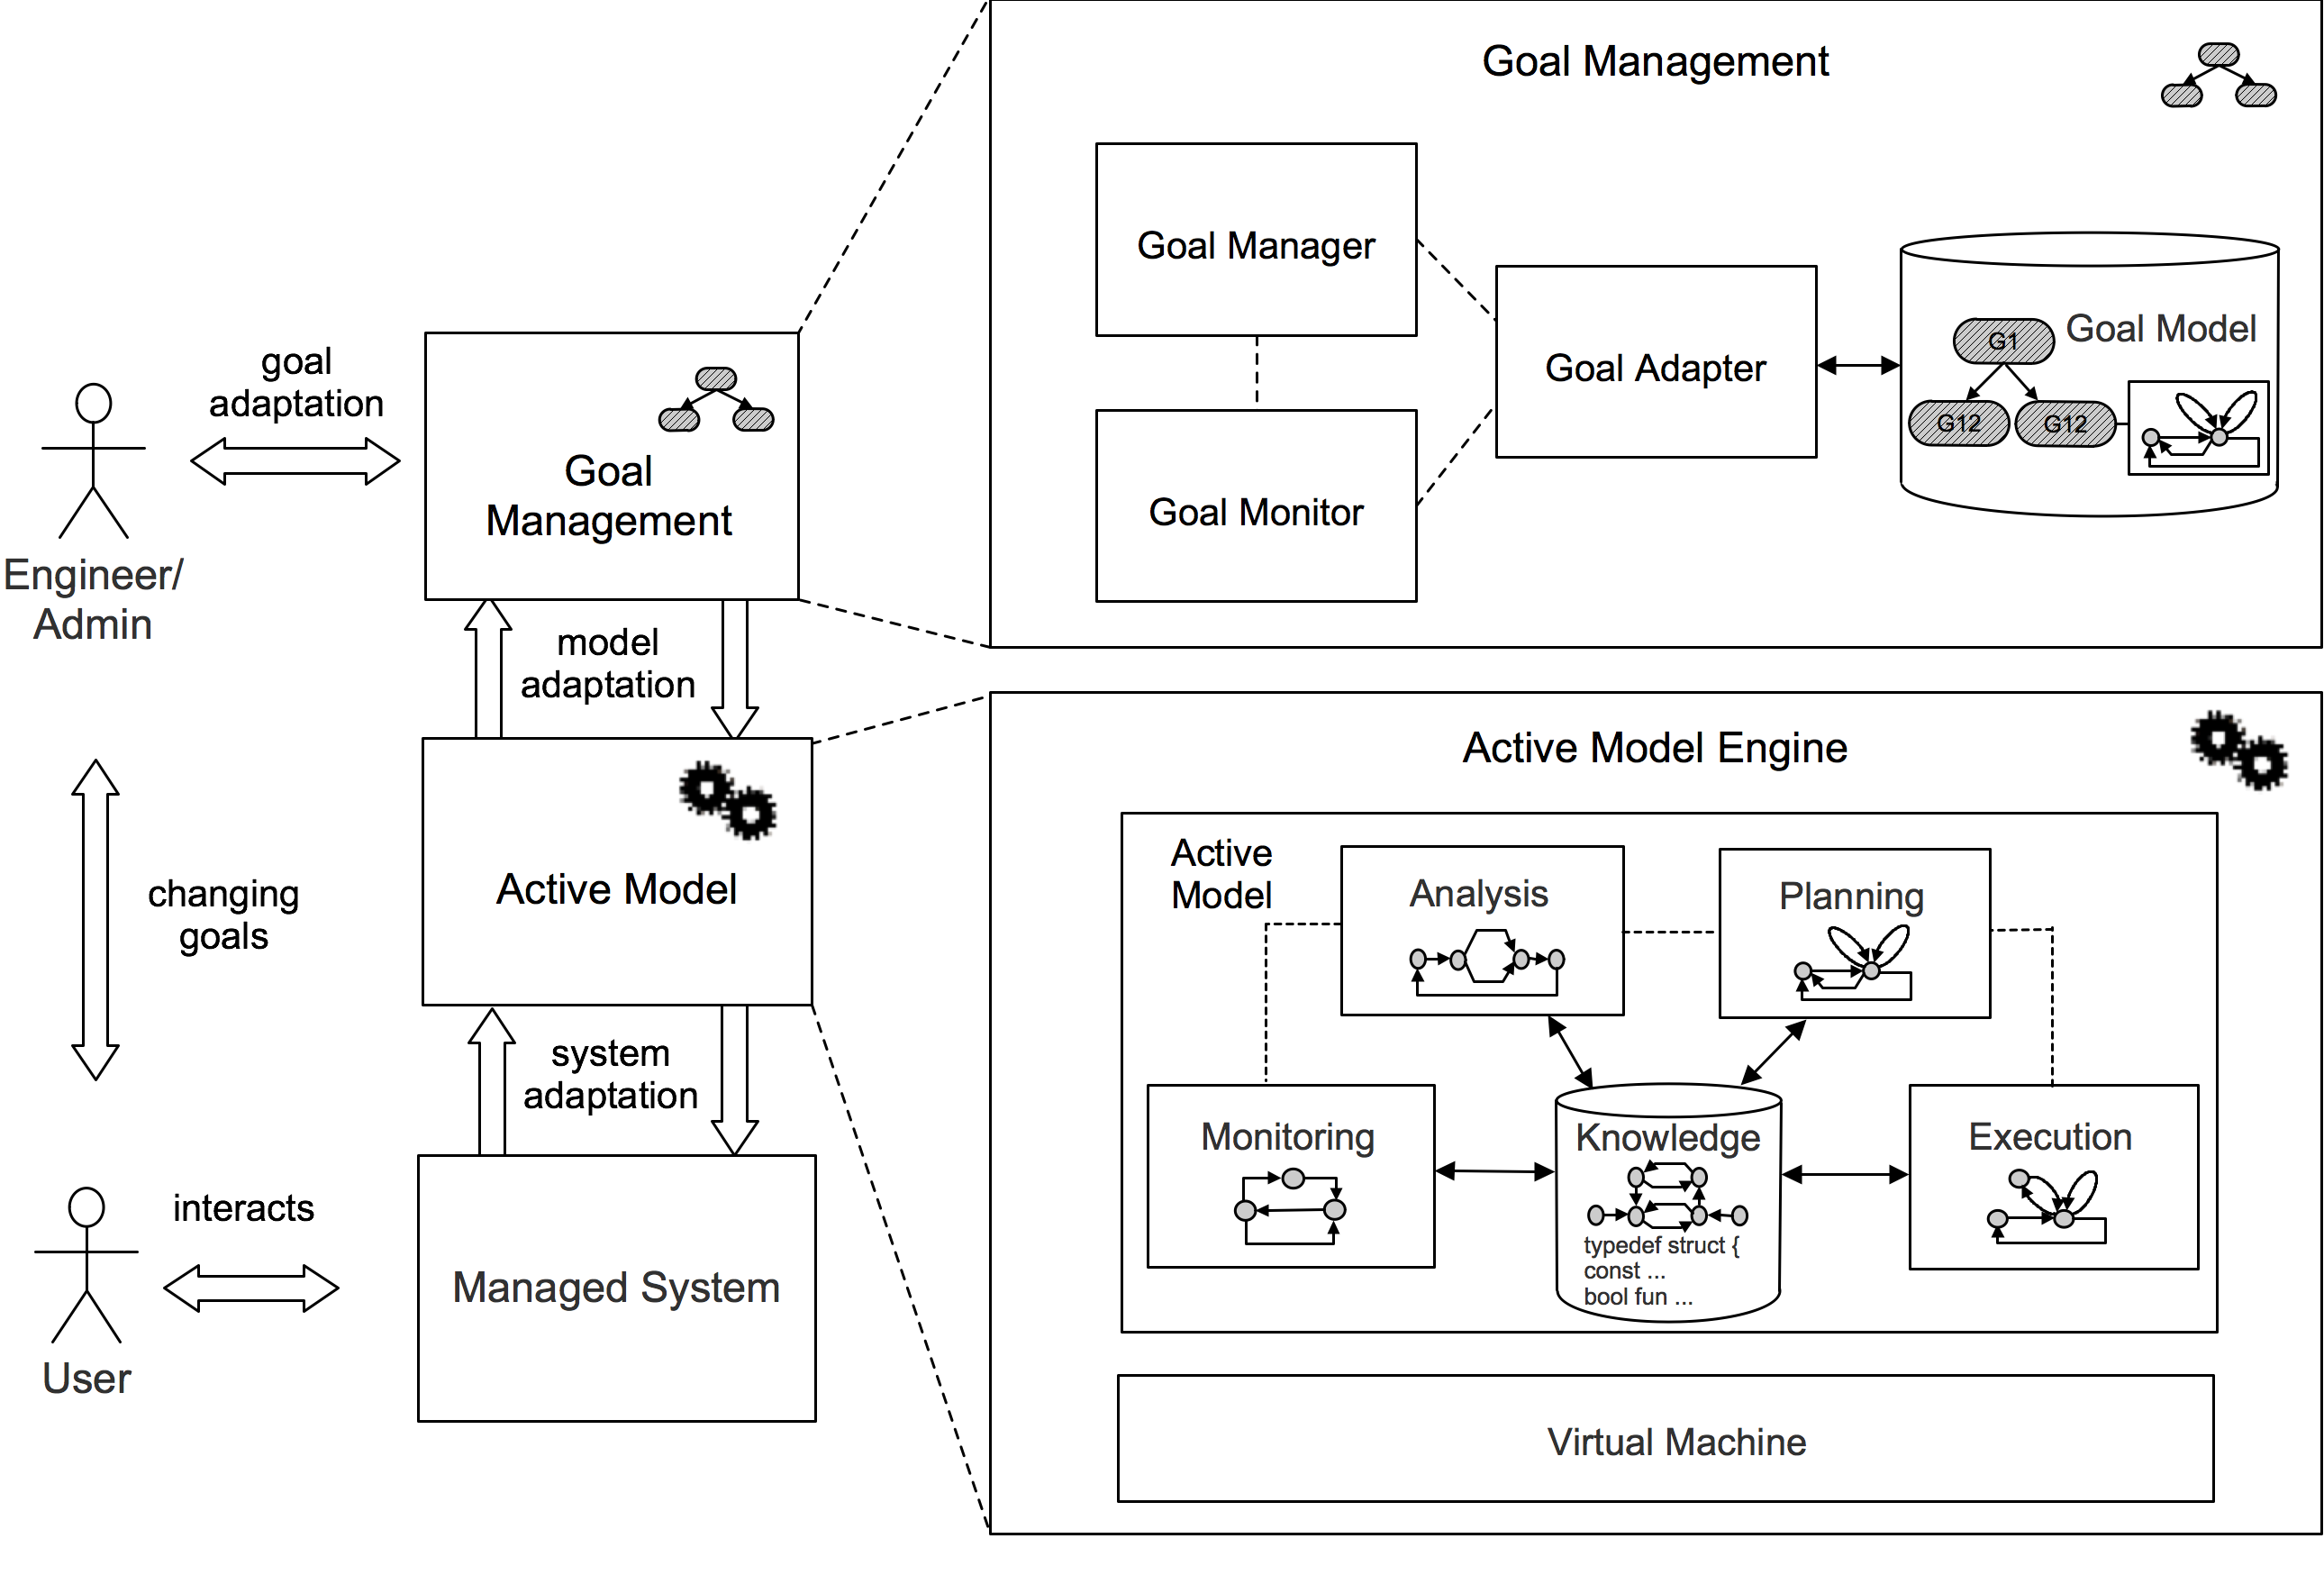
\includegraphics[width=0.7\textwidth]{figures/ActivFORMS-approach.png}
	\caption{ActivFORMS approach}\label{fig:activforms}
\end{figure}

Figure~\ref{fig:activforms} shows the primary modules of the ActivFORMS. The approach is in line with the three layered reference model for self-adaptive systems proposed by Kramer and Magee~\cite{Kramer2007:FOSE}. The managed system realizes the domain functionality for users. The active model consists of two parts: an integrated formal model that realises a feedback loop, i.e., the active model, and a virtual machine that can execute the active model. The active model monitors the managed system through probes and adapt the managed system through effectors. 

ActivFORMS supports feedback loops modelled using networks of timed automata~\cite{Alur1990}. A timed automaton is a finite-state machine that models a behaviour, extended with clock variables. Automata can synchronize through channels. There are two types of channels, binary channels and broadcast channels. For a binary channel, a sender x! can synchronize with a receiver x? through a signal. If there are multiple receivers x? then a single receiver will be chosen non-deterministically. The sender x! will be blocked if there is no receiver. On the contrary, a broadcast channel sends a signal to all the receivers, and if there is no receiver, the sender will not be blocked. Behaviour specifications can be complemented with expressions specified in a C-like language to define data structures (struct concept) and functions. Goals can be expressed in timed computation tree logic expressions (TCTL). TCTL expressions describe the state and path formulae that can be verified, such as reachability (a system should/can/cannot/... reach a particular state or set of states), liveness (something eventually will hold), etc. We use Uppaal~\cite{Behrmann2004}, a model checking tool that supports modelling of behaviours and verification of properties.

The goal management layer handles adaptation issues that cannot be performed by the current active model. The goal management consists of four parts, i.e., goal model, goal monitor, goal adapter and goal manager. The goal model represents the adaptation goals. ActivFORMS uses a AND-OR tree-based goal model to specify goals. The goals can be expressed as boolean expressions, and the goals at the bottom level of each subtree have associated models to realise adaptations. The goal monitor checks periodically the status of the goals and if any goal is violated, it notifies the goal adapter. The goal adapter is the heart of goal management. When the goal adapter receives a signal  from the goal monitor about a goal change, it consults the goal model and searches for a matching model that satisfies the changing situation. If the model associated with the changing goal differs from the currently deployed model, the goal adapter starts updating the current model with the new model at the virtual machine. If the model does not differ no further action is required. The goal manager offers support for three primary functions: inspecting the active model and its ongoing execution, monitoring and updating goals, and updating the goal model. In our current implementation, the ActivFORMS user interface connects with the goal managers of different system nodes. The user interface enables a software engineer, e.g., a system administrator, to operate the goal manger remotely.


%%%%%%%%%%%%%%%%%%%%%%%%%%%%%%%%%%
\section{Runtime Quantitative Verification}\label{sec:rqv}
%!TEX root = ../ENTRUST_TR.tex

\textit{Runtime quantitative verification} (RQV) \cite{Calinescu2012:CACM} is an approach to implementing the closed control loop of self-adaptive systems in which the adaptation decisions are driven by the continual verification of stochastic models. RQV was introduced in \cite{Calinescu2009:ICSE,Epifani2009:ICSE} and further refined in \cite{Calinescu2011:TSE,Filieri2011:ICSE,Johnson2013:CBSE}. 


Figure~\ref{fig:RQV} depicts the adaptation workflow of an RQV-based self-adaptive system. The approach involves monitoring the system (e.g., the UUV) and its environment continuously, to identify relevant changes and quantify them using fast on-line learning techniques. When these changes are significant and/or periodically, an RQV step is triggered, to identify which scenario the system operates in, and to select the associated model from a family of system models (i.e., a \emph{parametric model}) that correspond to different such scenarios. The selected model is then analysed using quantitative verification, to identify and/or predict violations of QoS requirements such as response time, availability and cost. When QoS violations are identified or predicted, the verification results support the selection of a new set of values for the configurable system parameters, so that enforcing this new configuration is \emph{guaranteed} to restore or maintain compliance with QoS requirements, respectively.

\begin{figure}[t]
\centering
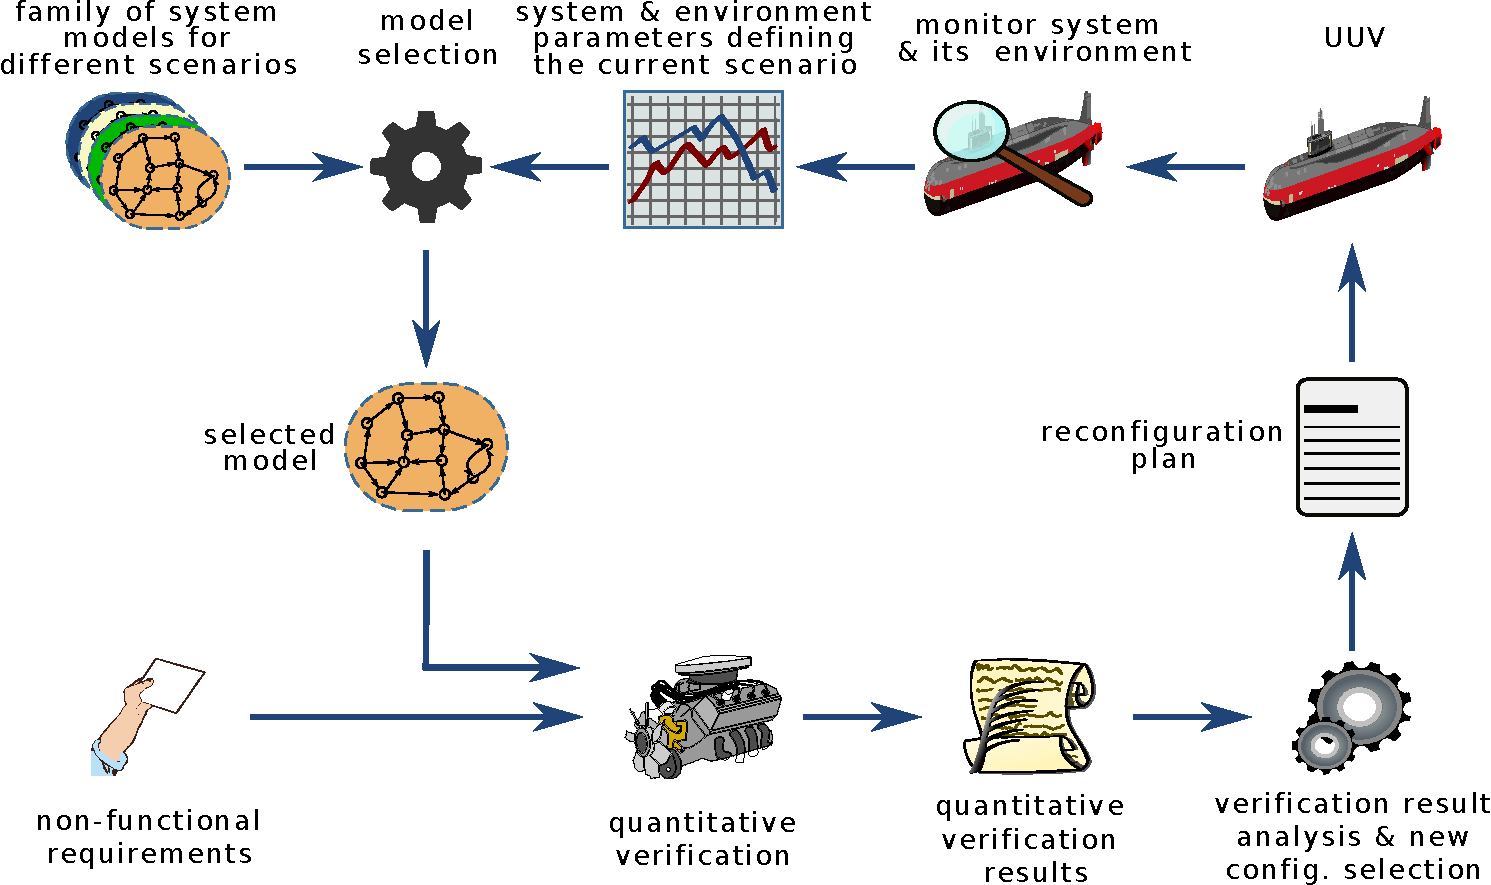
\includegraphics[width=0.75\hsize]{figures/rqv.pdf}
\caption{RQV-based self-adaptive system}
\label{fig:RQV}

\vspace*{-2mm}
\end{figure}

%%%%%%%%%%%%%%%%%%%%%%%%%%%%%%%%%%
\section{Implementation}\label{sec:implementation}
\input{sections/Implementation.tex}

%%%%%%%%%%%%%%%%%%%%%%%%%%%%%%%%%%
\section{Methodology}
TBC

%%%%%%%%%%%%%%%%%%%%%%%%%%%%%%%%%%
%%%%%%%%%%%%%%%%%%%%%%%%%%%%%%%%%%
%%%%%%%%%%%%%%%%%%%%%%%%%%%%%%%%%%
\bibliography{entrust}
\bibliographystyle{ieeetr}

\end{document}